% !TeX root =  main.tex

\section{Functions}

\subsection{Basic Concepts}
\begin{definition}
  A \textbf{relation} is a set of ordered pairs. The set of the first components of each ordered pair is called the \textbf{domain} and the set of the second components of each ordered pair is called the \textbf{range}.

  A \textbf{function} is a relation that assigns each element in the domain a unique element in the range.

  An arbitrary value in the domain is often represented by the lowercase letter $x$ which is called an \textbf{independent variable}.
  An arbitrary output is often represented by the lowercase letter $y$ which is called a \textbf{dependent variable}.
  
  Each value in the domain is also known as an input value. Each value in the range is also known as an output value.
\end{definition}

\begin{example}
  The relation 
  \[\{(1,2),(2,4),(3,6),(4,8),(5,10)\}\]
  is a function.
  
  The domain is $\{1,2,3,4,5\}$. The range is $\{2,4,6,8,10\}$.
\end{example}

If a function has $x$ as the independent variable and $y$ as the dependent variable, then we often say that $y$ is a function of $x$.

\begin{example}
  In a grocery store, if we take items as the domain, and prices as the range, then the relation is a function. Because each item must have a unique price.
  
  However, if we take prices as the domain and items as the range, then the relation is not a function in general. Because there are often multiple items with the same price.
  
  Those two relations may be described as the follow.
  Price is a function of item. Item is not a function of price.
\end{example}

  In mathematics, a function is often named by letters, such as $f$, $F$, $p$, or $q$. To describe a function named $f$, we often use the equation notation $y=f(x)$ which means that $f$ assigns to the input $x$ the output value $y$. Here $f(x)$ is read as $f$ of $x$ or $f$ at $x$. The notation $f(x)$ is known as the function notation which represents the output of the function $f$ when the input is $f$. 


\subsection{Domains and Ranges}


\section*{Exercises}

\begin{exercise}
    Find the vertex, focus, and directrix of the parabola. Sketch the graph.\\
    \begin{enumerate*}
        \item $x^2=-8y$.
        \item $y^2=12x$.
        \item $x^2+6y=0$.
        \item $2x-y^2=0$.
    \end{enumerate*}
\end{exercise}
\vspace*{10\baselineskip}

\begin{exercise}
    An equation of an ellipse is given. Find the center, vertices, and foci of the ellipse, and the lengths of the major and minor axes. Sketch the graph.\\
    \begin{enumerate*}
        \item $\dfrac{x^2}{9}+\dfrac{y^2}{25}=1$.
        \item $\dfrac{y^2}{9}+\dfrac{x^2}{25}=1$.
        \item $9x^2+25y^2=1$.
        \item $25x^2+9y^2-16=0$.
    \end{enumerate*}
\end{exercise}
\vspace*{10\baselineskip}

\begin{exercise}
    An equation of an ellipse is given. Find the center, vertices, foci, and asymptotes of the hyperbola. Sketch the graph.\\
    \begin{enumerate*}
        \item $\dfrac{x^2}{9}-\dfrac{y^2}{25}=1$.
        \item $\dfrac{y^2}{9}-\dfrac{x^2}{25}=1$.
        \item $9x^2-25y^2=1$.
        \item $25x^2-9y^2-4=0$.
    \end{enumerate*}
\end{exercise}
\vspace*{10\baselineskip}

\begin{exercise}
    Find an equation for
    the conic section with the given properties.
    \begin{enumerate}
        \item The parabola with vertex at the origin and focus $(0, 5)$.
        \item The parabola with vertex at the origin and the directrix $x=-2$.
        \item The ellipse with vertices $(\pm 2, 0)$ and foci $(\pm 1, 0)$.
        \item the ellipse with foci $(0,\pm 3)$ and the eccentricity $e=\frac34$.
        \item The hyperbola with foci $(0,\pm 3)$ and vertices $(\pm 2, 0)$.
        \item The hyperbola with foci $(\pm 5, 0)$ and asymptotes $y=\pm\frac34$.
    \end{enumerate}
\end{exercise}

\begin{exercise}
    Find an question for the conic section with the given graph.
    \begin{enumerate}
        \item \mbox{}

        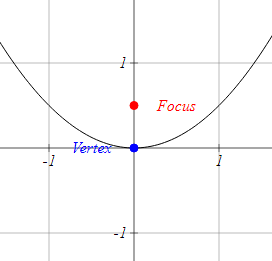
\includegraphics[width=0.3\textwidth]{figs/ParabolaEqFromGraph.png}
        \item \mbox{}

        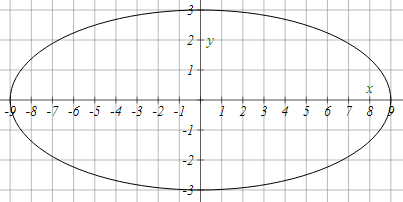
\includegraphics[width=0.4\textwidth]{figs/EllipseEqFromGraph.png}
        \item\mbox{}

        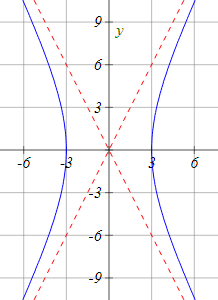
\includegraphics[width=0.3\textwidth]{figs/HyperbolaEqFromGraph.png}
    \end{enumerate}
\end{exercise}
